% IEEE standard conference template; to be used with:
%   spconf.sty  - LaTeX style file, and
%   IEEEbib.bst - IEEE bibliography style file.
% --------------------------------------------------------------------------

\documentclass[letterpaper]{article}
\usepackage{spconf,amsmath,amssymb,graphicx,float,enumitem,url,dblfloatfix}

% Example definitions.
% --------------------
% nice symbols for real and complex numbers
\newcommand{\R}[0]{\mathbb{R}}
\newcommand{\C}[0]{\mathbb{C}}

% bold paragraph titles
\newcommand{\mypar}[1]{{\bf #1.}}

% Title.
% ------
\title{Optimization and parallelization of diffusion solvers\\
using alternating direction implicit and random walk methods}
%
% Single address.
% ---------------
\name{Samuel Maloney} 
\address{Department of Mathematics\\ETH Z\"urich\\Z\"urich, Switzerland}

% For example:
% ------------
%\address{School\\
%		 Department\\
%		 Address}
%
% Two addresses (uncomment and modify for two-address case).
% ----------------------------------------------------------
%\twoauthors
%  {A. Author-one, B. Author-two\sthanks{Thanks to XYZ agency for funding.}}
%		 {School A-B\\
%		 Department A-B\\
%		 Address A-B}
%  {C. Author-three, D. Author-four\sthanks{The fourth author performed the work
%		 while at ...}}
%		 {School C-D\\
%		 Department C-D\\
%		 Address C-D}
%

\begin{document}
%\ninept
%
\maketitle
%


% ----------------------------------------------------------------------
\begin{abstract}
Optimized and parallelized code for numerical simulation of the diffusion equation is presented. Two different algorithms, Alternating Direction Implicit (ADI) and Random Walk (RW) are studied. The algorithms are implemented in C++ and verified against an analytic solution, and then scalar optimizations, Advanced Vector Extensions (AVX) vectorization, and OpenMP parallelization are carried out. Benchmarking tests are conducted on the Piz Daint cluster to determine single-core performance and runtime improvements, as well as strong and weak scaling characteristics on multiple cores of a single node. Approximate performance gain of 4.8X for ADI, and maximal runtime speedups of approximately 9.4X and 58X for ADI and RW respectively are observed. Acceptable OpenMP scaling is found for both algorithms in strong and weak scaling analyses.
\end{abstract}


% ----------------------------------------------------------------------
\section{Background}\label{sec:background}

\mypar{Motivation} 
Diffusion is the process by which a~quantity of interest spreads from regions of high density to regions of low density and is integral in the study of fluids. Diffusion terms arise in all numerical models of computational fluid dynamics, which are used for such problems as aerodynamic design, turbine flows, chemical reaction mixing, and many others. Efficient and accurate simulation codes for diffusion are thus of great importance in many fields.

In this study, two different algorithms to simulate the diffusion process, Alternating Direction Implicit (ADI) and Random Walk (RW), were implemented, optimized, and parallelized. The mathematical formulations for diffusion in general and for each of these two methods specifically are presented next.

\mypar{Mathematical Formulation}
The process of diffusion is driven by a conentration gradient according to the diffusion equation:
\begin{equation}
\frac{\partial \rho(\mathbf{r},t)}{\partial t} = D\Delta\rho(\mathbf{r},t)
\label{diff}
\end{equation}
where $\rho(\mathbf{r},t)$, with position $\mathbf{r}$ at time $t$, is the quantity of interest and $D$ is the diffusion constant and is a given value for the system. For this study, homogeneous Dirichlet boundary conditions are used at all boundaries. The initial density distribution used for this study is:
\begin{equation}
\rho(x,y,0)=\sin(\pi x)\sin(\pi y)
\end{equation}
and its corresponding analytic solution, which was used for verification, is:
\begin{equation}
\rho(x,y,t)=\sin(\pi x)\sin(\pi y)e^{-2D\pi^{2}t}
\label{analytic}
\end{equation}
The studied simulation domain is a unit square with $x$ and $y$ each ranging from $0$ to $1$, which is discretized using a uniform grid such that $\delta h=\delta x=\delta y$. A superscript $n$ is used to denote the timestep $t_n=n\delta t$ and subscripts $i$ and $j$ to denote the indices of the nodes in the mesh $x_i=i\delta x$ and $y_j=j\delta y$ such that $\rho_{i,j}^{n}=\rho(x_i,y_j,t_n)$.

\mypar{Alternating Direction Implicit}
The ADI method is an operator splitting scheme based on finite difference discretizations of the derivatives. It works by splitting each timestep into two half timesteps, in the first of which the time integration is carried out implicitly in the $x$-direction and explicitly in the $y$-direction, and in the second half time step the directions are switched such that the integration in the $x$-direction is explicit and in the $y$-direction is implicit.

Using a second order centered approximation for the spatial derivative in Eq. \eqref{diff} means that each implicit integration step requires only the solution of a tridiagonal linear system, for which the Thomas Algorithm (for formulation see \cite{thomas}) can be used to efficiently compute the result. These tridiagonal systems can be found by considering the discretization equations:
\begin{equation}
\rho_{i,j}^{n+\frac{1}{2}}=\rho_{i,j}^n+\frac{D\delta t}{d\delta x^2}(\rho_{i-1,j}^{n+\frac{1}{2}}-2\rho_{i,j}^{n+\frac{1}{2}}+\rho_{i+1,j}^{n+\frac{1}{2}})
\end{equation}
\begin{equation}
\rho_{i,j}^{n+1}=\rho_{i,j}^{n+\frac{1}{2}}+\frac{D\delta t}{d\delta x^2}(\rho_{i,j-1}^{n+1}-2\rho_{i,j}^{n+1}+\rho_{i,j+1}^{n+1})
\end{equation}
which can be rewritten in the form $\mathbf{A}\rho^*=\rho^{*-\frac{1}{2}}$ where $\mathbf{A}$ is the tridiagonal matrix to be solved at each half timestep.

\mypar{Random Walk}
Diffusion can also be simulated by tracking the random motion of a set of $M$ identical particles with no inertia. A probability $\lambda=D\delta t/\delta x^2$ is defined, such that at each time step, each particle has a $1-4\lambda$ probability of remaining in the same position. If it does not stay, it is then moved to one of the four neighbouring nodes, with an equal probability of moving in any direction. Clearly, one requires $\lambda<1/4$ to maintain a positive probability of staying.

The initial condition for the number of particles at each grid point $m_{i,j}$ is given as:
\begin{equation}
m_{i,j}^0=\left \lfloor{\frac{M\rho(x_i,y_j,0)}{\iint_\Omega \rho(x,y,0) \,\mathrm{d}x\,\mathrm{d}y}}\right \rfloor 
\end{equation}
And the approximate solution after a given timestep can then be calculated as:
\begin{equation}
\rho_{i,j}^n=\frac{m_{i,j}^n}{M}\iint_\Omega \rho(x,y,0)  \,\mathrm{d}x\,\mathrm{d}y
\end{equation}

% ----------------------------------------------------------------------
\section{Baseline Implementation}\label{sec:baseline}

In this section, the basic implementation and verification of the described algorithms is presented. All code is based on the {\tt Diffusion2D} class structure of the solution code provided with the course exercises. All code for each version of the class is contained within a single .cpp source file, which requires the user defined header files \textit{timer.hpp} and \textit{tsc\_x86.hpp} for measuring runtime in seconds and cycles respectively. The \textit{timer.hpp} file is from the HPCSE I course exercises, and the \textit{tsc\_x86.hpp} file is from the exercises of the How to Write Fast Numerical Code course at ETH.

The programs take arguments to set the diffusion constant $D$, size $N$ of one dimension of the grid, timestep $\delta t$, number of repititions $n_{runs}$ to run the simulation, and the number of timesteps $n_{steps}$ to run each simulation for. The RW codes also take a value for the numer of particles $M$ in the simulation. For all codes the values for $n_{runs}$ and $n_{steps}$ are optional, and default to $n_{runs}=1$ and $n_{steps}=0.1/\delta t$ respectively. The ordering of these input arguments can be displayed by running the program with no arguments.

For each simulation run, a new {\tt Diffusion2D} class object is initialized, with one-time initialization routines happening outside of the timing structures. Once initialization is complete, the simulation is is run to completion by a single call to the {\tt run\_simulation} function, and this call is the only part of the program which is timed and contains all code which will be optimized. 

\mypar{ADI}
An order verification study (OVS) of the ADI code in both spatial and temporal dimensions was performed by comparing the simulation results to the analytic solution in Eq. \eqref{analytic}. The results can be seen in Fig. \ref{fig:OVS_ADI} and show the implementation to be second order accurate in both space and time, as expected for this discretization scheme.

The ADI algorithm complexity should be $O(N^2)$ as it does a constant number of operations for updating the value at each point in the grid. Its runtime scaling (see \ref{subsec:ADI_results}, Fig. \ref{fig:runtime_ADI}) is found to agree with this expected complexity.

\begin{figure}\centering
  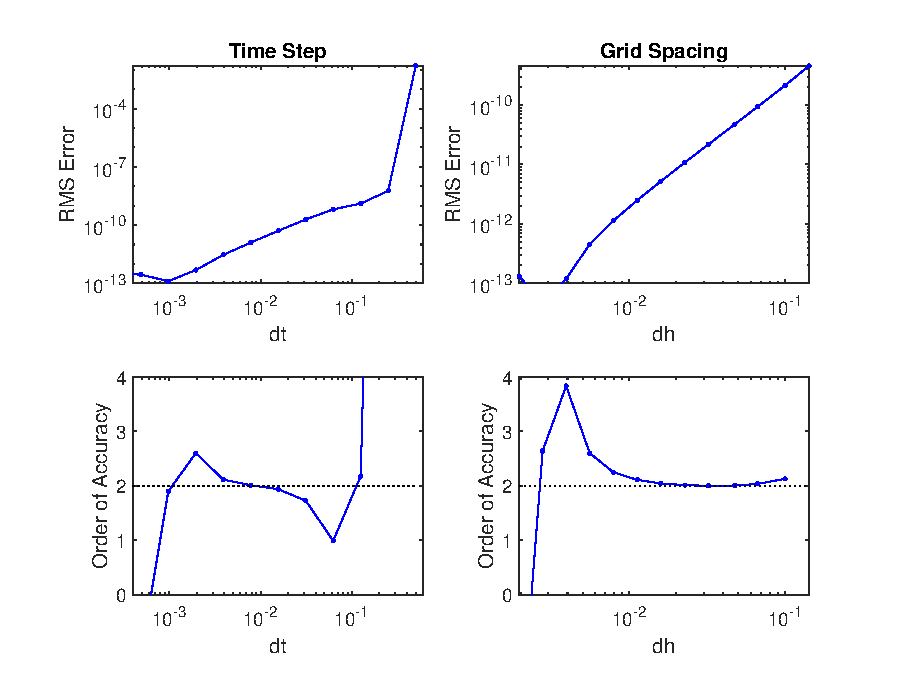
\includegraphics[width=\linewidth]{./plots/OVS_ADI.eps}
  \caption{Order verification study of the ADI code in space and time.}
  \label{fig:OVS_ADI}
\end{figure}

For performance analysis, the cost of the ADI code is defined as the number of floating point operations (FLOPs) including additions, multiplications, and, for the baseline implementation only, divisions. Moreover, the data movement in bytes between various levels of cache was measured using the Hardware Performance Counter (HWPC) functionality in CrayPat to quantify the operational intensity.

The results of a roofline analysis are shown in Fig. \ref{fig:roofline_ADI_serial} for the baseline code. Three data series are presented, which use the same performance data but compute the operational intensity with respect to different levels of the cache heirarchy. The implementation appears compute bound with respect to memory tranfers with RAM, but for large $N$ it becomes clearly memory bound at higher levels of the cache, albeit with still siginificant room to improve towards the memory bandwidth rooflines. Maximum performance of 0.734 FLOPs/cycle, or 18\% of peak scalar performance is observed. On the test machine, with an Intel Haswell central processing unit (CPU), the peak performance is calculated by considering the maximum throughput of 2 fused multiply add (FMA) instructions per cycle, giving 4 total FLOPs per cycle. Data for the cache bandwidths used in this (and subsequent) roofline plots was obtained from \cite{7_cpu} and \cite{manual_intel}.

\begin{figure}\centering
  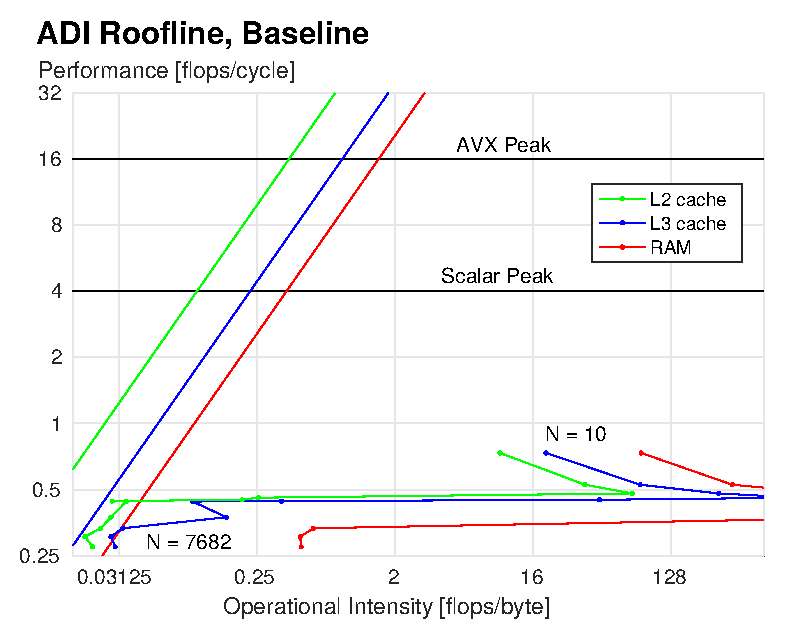
\includegraphics[width=\linewidth]{./plots/roofline_ADI_serial.eps}
  \caption{Roofline analysis of the ADI baseline code.}
  \label{fig:roofline_ADI_serial}
\end{figure}

\mypar{RW}
One of the most important aspects of the RW implementation is the choice of Pseudorandom Number Generator (PRNG) used. Knowing that parallelization would eventually be necessary, the SITMO PRNG \cite{sitmo} was initially selected. It claims to be faster than the C++ Mersenne Twister, passes all BigCrush test in the TestU01 framework, and provides easy access to many non-overlapping streams which would be useful for later parallelization.

For the baseline implementation only, the code loops over all nodes and then at each node loops over all particles at that node. For each particle a random number is generated to determine if it stays or in which direction it should move. An OVS for the baseline RW code is shown in Fig. \ref{fig:OVS_RW_1} with respect to the number of particles in the simulation, again comparing to the analytic solution. This study confirms the baseline to converge as $\sqrt{M}$ as expected from theory.

As explained in section \ref{subsec:RW_method}, algorithmic changes were made during later optimizations of the RW code, and so additional OVSs were carried out on these later versions to ensure they remained correct. Results for these verifications are shown in Fig. \ref{fig:OVS_RW_2} and confirm that the $\sqrt{M}$ convergence is preserved.

\begin{figure}[!b]\centering
  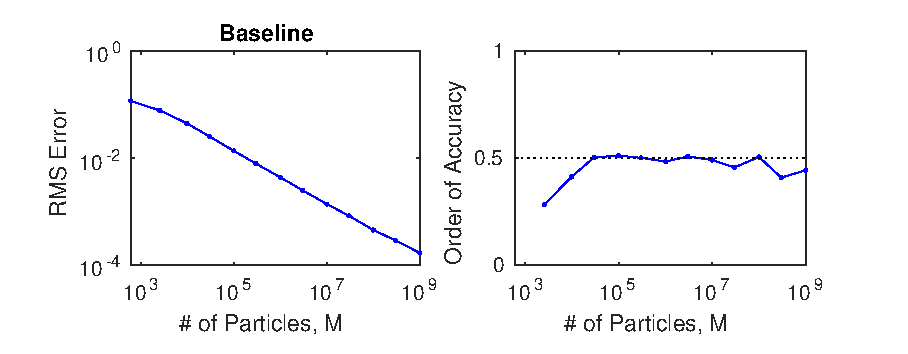
\includegraphics[width=\linewidth]{./plots/OVS_RW_1.eps}
  \caption{Order verification study of the baseline RW code for the number of simulation particles.}
  \label{fig:OVS_RW_1}
\end{figure}

\begin{figure}\centering
  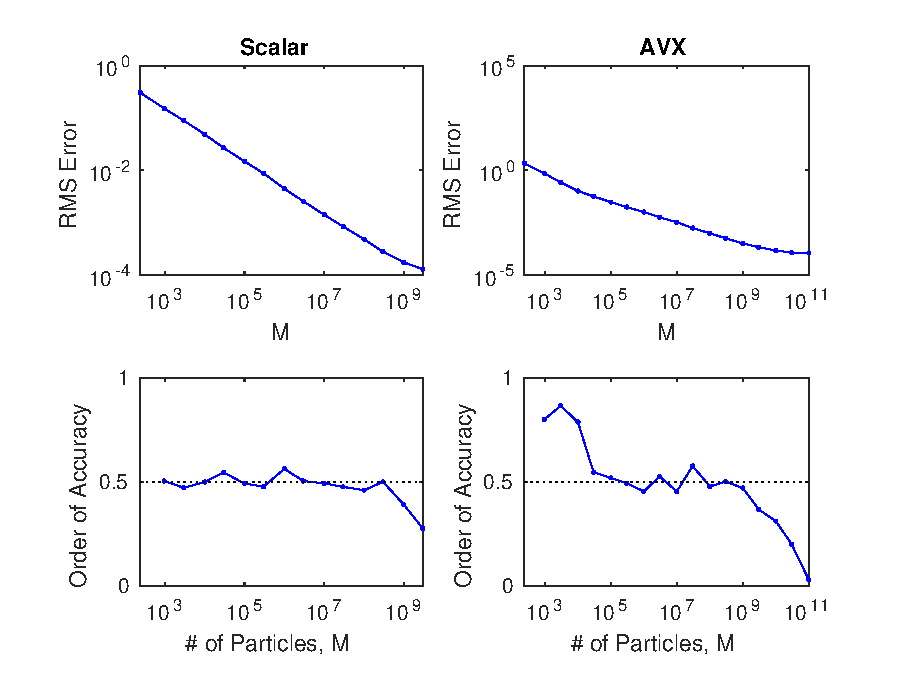
\includegraphics[width=\linewidth]{./plots/OVS_RW_2.eps}
  \caption{Order verification studies of the optimized RW codes for the number of simulation particles.}
  \label{fig:OVS_RW_2}
\end{figure}

Complexity for the RW method depends on which version is being considered. The baseline implementation should scale as $O(M)$, where $M$ is the number of particles in the simulation. This is because a random number must be generated for each particle in the simulation to determine it's movement for a given timestep, independent of how many grid points there are in the simulation. The later versions
that use a binomial random variable (see \ref{subsec:RW_method}) to simulate particle movement scale as $O(N^2)$ because exactly four such random variables must be evaluated for each grid point, independent of the number of particles in the simulation.

Measurements of this runtime scaling (see \ref{subsec:RW_results}, Fig. \ref{fig:runtime_RW}) confirm $O(N^2)$ for all versions of the code. This is as expected for the optimized versions, but also matches for the baseline version, since the number of particles was chosen as $M=1000N^2$, meaning the $O(M)$ complexity is equivalent to $O(N^2)$ complexity for these baseline experiments as well.


% ----------------------------------------------------------------------
\section{Optimization Methods}\label{sec:method}

In this section the main optimizations that were undertaken are explained. Optimizations of the ADI and RW methods are discussed in separate subsections. For each algorithm, the optimizations are broken down into three revisions: the \textit{Scalar} revision contains only optimizations that do not involve manual vectorization or parallelization (although it is noted that the compiler was not prevented from vectorizing, so this naming scheme is not meant to imply that the machine code is not vectorized, only that it was not manually attempted at this stage); the \textit{AVX} revision then adds manual vectorization using intrinsics; and the \textit{OpenMP} revision add parallelization using OpenMP to run on a single full XC50 node of Piz Daint.

\subsection{ADI}\label{subsec:ADI_method}

\mypar{Scalar}
Several different types of optimizations were included in this revision. Firstly, the number of operations required was greatly reduced by precomputing several factors needed for the Thomas algorithm that were the same for each row/column and timestep. This required an additional two vectors of length $N$ to store the precomputed values, but greatly reduced the FLOP count overall, and in particular removed all division operations from the simulation loop.

Secondly, unrolling of the outer loops was performed to take advantage of the spatial locality in the algorithm. It achieves a speedup because updating the values for each row/column requires the values from the immediately adjacent rows/columns, so by unrolling the loop we expose independent operations in adjacent rows which use the same data, thus decreasing the data movement required and increasing Instruction Level Parallelism (ILP). It was decided to unroll by a multiple of four, in preparation for vectorization with AVX, and unrolling factors of four, eight, and twelve were tested, with a factor of eight determined to be optimal on the test system.

Lastly, Single Static Assignment (SSA) was introduced throughout the code to promote optimal register allocation by the compiler for all reused data values and computations.

\mypar{AVX}
Manual vectorization of the code was carried out by leveraging Intel fused-multiply-add (FMA) and advanced vector extension (AVX) intrinsics. In the final version of this code, only the loop over the columns was manually vectorized, as nothing that was attempted to the row loop was able to reduce the runtime. This is mostly due to the row-major storage order of C++ arrays, which mean that data for adjacent columns is nicely aligned for loading to and from AVX vectors, but the data from adjacent rows requires some sort of gathering and scattering operations to fill the vectors with the correct data. Several methods of achieving this were tested, but were found ot be slower than simply letting the compiler handle the scalar code.

The first method attempted involved storing the half-timestep result in transposed form, such that both loops were loading their data column-wise, thus requiring only the single scatter operation for each vector of values updated, abeit for both loops, rather than the one scatter and three gather operations that would have been required to read and store in the row-wise loop. The second method attempted involved unrolling the inner row loop by a factor of four, such that the full vectors of data from each load operation could be used, rather than just the single value used from each load operation in a gather. This reduced the number of load instructions required by a factor of four, but does replace them with a number of shuffle and permute operations to arrange all of the loaded data properly into vectors for the computations (AVX transposition code based on \cite{transpose}).

One last thing that was attempted at this stage was unrolling of the vectorized inner column loop in an attempt to improve piplining of operations. An unrolling factor of three was selected as it was the largest factor for which the number of required AVX vectors in the code did not exceed the number of available AVX registers on the CPU. In this way, load instructions for data for future iterations were interleaved with computations for current iterations, but unfortunately no improvement in runtime was attained, and so this unrolling of the inner loop was not included in the final code for this revision.

Implementations for the required scatter, gather, and rearranging operations were hand coded and optimized using throughput, latency, and execution port data from Agner Fog's tables \cite{Agner}, which were also used for analysis of instruction level dependencies in the attempts to improve piplining.

\mypar{OpenMP}
Initial parallelization of the ADI code with OpenMP was quite straightforward. The code was restructured slightly, such that instead of a loop in the main function calling an {\tt advance} function for each iteration, the loop was placed directly around the simulation code inside of a {\tt run\_simulation} function, as mentioned in section \ref{sec:baseline}. This allowed for a single {\tt omp parallel} region to be created at the beginning of the simulation that would only be exited upon completion, preventing joining and spawning of threads between iterations and removing OpenMP overhead from within the loop. After that, simple parallelization was achieved with {\tt omp for} on both loops, using a {\tt no wait} clause on the second loop because synchronization would already be achieved by the {\tt omp single} used for updating the step counter only once at the end of each iteration.

However, one major issue which remained with this initial implementation was false sharing. Although the individual threads never need to write to exactly the same entries of the array, they are often writing to nearby entries at the boundaries of their working sets. This means that the boundaries of each working set should be cache line aligned in order to prevent false sharing between threads. To attain this, a~check was added to the code requiring that the number of grid points $N$ be a multiple of eight, since there are eight doubles in a 64 B cache line. An {\tt aligned\_alloc} was then used to allocate 64 B aligned memory for storage, and as the outer loops were already unrolled by a factor of eight this ensured that each thread's working set did not share cache lines with its neighbours.

Binding of threads to cores was also investigated by setting the {\tt KMP\_AFFINITY} environment variable provided by the intel compiler environment \cite{affinity}. Values of {\tt compact} and {\tt scatter} were tested, with {\tt scatter} found to give faster runtimes and so it was used for the final OpenMP benchmarking tests.


\subsection{RW}\label{subsec:RW_method}

\mypar{Scalar}
The main optimization of this version lies in no longer looping over every particle and indivdually computing a random number to determine its potential movement, but rather looping only over each node and generating four binomially distributed random numbers to determine the ensemble number of particles that move in each direction. This makes the runtime scaling independent of the number of particles in the simulation, allowing much higher accuracy simulations  without prohibitively increasing the runtime. It is noted that because the sum of the four binomially distributed numbers can be greater than the actual number of particles on the node, particularly for small $M$, a check was added to the code to handle negative nodal values during simulation, but they can still show up as negative values in the final density solution.

A further optimization involved moving the particle to density computation out of the simulation loop and into its own function, such that the conversion was not calculated on each time step, but manually called after completion of the simulation to compute the final approximate solution.

\mypar{AVX}
Vectorization of the code was performed using Single Instruction Multiple Data (SIMD) intrinsics. However, it was quickly discovered that the AVX intrinsics had only a minimal speedup because the PRNG itself was where most of the runtime was spent, and so vectorized PRNG options were investigated. Intel's Math Kernal Library (MKL) Vector Statistics (VS) package implements a~Streaming\linebreak SIMD Extension (SSE) version of its fast mersenne twister PRNG \cite{SFMT}, and so this was integrated with the AVX intrinsics to create a fully vectorized version of the code.

Because the RW algorithm updates the four neighbouring nodes for any given one being looped over, it was found to be faster if only six nodes were looped over at a time, instead of the maximum eight which would correspond to a full AVX vector of 32-bit integers. This allowed the values being added to the neighbouring nodes to be cleverly aligned within the AVX vectors and added using basic ADD intrinsics, one on top of the other, and eliminated a~small dependency chain of loads and stores that occurred when the loop was originally unrolled by a full factor of eight.

\mypar{OpenMP}
Again because of the RW algorithm updating the nodes neighbouring the ones being looped over, the main challenge for OpenMP parallelization was preventing race conditions at the boundaries of each thread's working set. To this end, an array of {\tt omp\_mutex} objects (from the C++ class implementation provided in HPCSE I) was introduced, with each lock in the array matching to one of the working set boundaries. Working set indices for each thread were manually computed and the inner for loop was separated into three parts, one each for the first two and final two rows in each working set, which are the ones that have overlap with neighbouring threads, and one for the interior cells that do not have any possible race condition. Each thread then must acquire a lock before entering one of its boundary loops, with the lock for loop over the first rows of one thread corresponding to the lock for the final rows of the previous thread to prevent race conditions.

Each thread also requires independently generated random numbers, and so each has its own PRNG stream which is made to be {\tt threadprivate}. The streams are ensured to be non-overlapping by using the skip ahead functionality provided by the MKL VS library, with the number of entries in the sequence to be skipped being calulated from the user supplied number of grid points and timesteps.


% ----------------------------------------------------------------------
\section{Optimization Results}\label{sec:results}

In this section the results of numerical benchmarks of the code at various stages are presented. Runtime and scaling experiments were performed for both algorithms, as well as performance and roofline analyses for ADI.

\mypar{Experimental setup}
All data was collected using a single XC50 node of Piz Daint, which has a 12 core Intel Xeon E5-2690 v3 running at 2.6 GHz \cite{daint}. Each physical processor core has a 64 KB L1 cache split equally into two 32 KB data and instruction caches, and a 256 KB unified L2 cache \cite{cpu_world}. The 30 MB L3 cache is shared between all cores \cite{ark_intel}, and there is 24.9 GB/s bandwidth to main memory \cite{7_cpu}. The Intel C++ Compiler v17.0.1 was used with "-O3 -std=c++11 -DNDEBUG -march=core-avx2 -fno-alias -qopenmp -mkl" flags. The Intel time stamp counter (TSC) was used for runtime measurements and CrayPat was used for cache miss measurements.

The inputs are the number of grid points in the domain discretization, the timestep between iterations, and the number of timesteps computed. We used grids of various sizes, up to $N\times N=7680\times7680$. The diffusion constant $D=1$ is used for all simulations, and for RW simulations $M=1000N^2$ particles was used. For ADI, $1000$ timesteps were computed, and for RW $50$ timesteps were computed to achieve a reasonable runtime for measurements. Each simulation was repeated $10$ times, with the minimum cycle count used for the runtime and the average cache misses used for the memory transfer (the average is used only because it would have prohibitively time-consuming to measure minimum values with CrayPat).

All experiments were performed with warm cache. This is largely to simulate real world usage scenarios, where the simulation would most likely be performed immediately after initialization while the data is still potentially in cache, exactly as in these experiments. It is noted, however, that the initial cache state should have little effect on the results in either case, as the effects will be amortized over the number of iterations performed, and should become negligible for the relatively large number of iterations used.

\begin{figure}\centering
  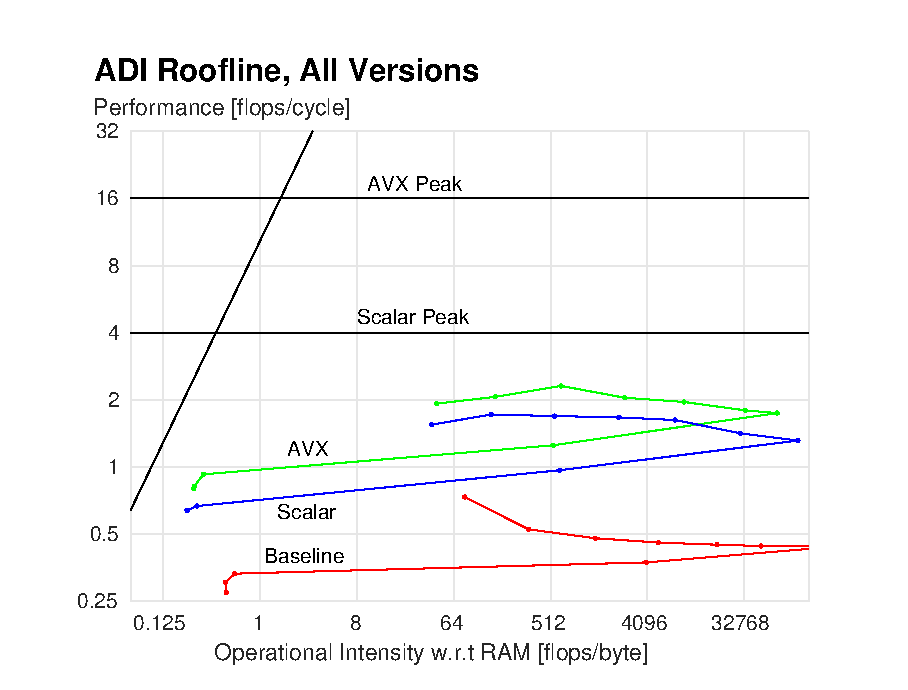
\includegraphics[width=\linewidth]{./plots/roofline_ADI_all.eps}
  \caption{Roofline analysis of the ADI code.}
  \label{fig:roofline_ADI_all}
\end{figure}

\subsection{ADI}\label{subsec:ADI_results}
Roofline, runtime, and scaling experiments were conducted on the ADI code, the results of which are presented next.

\mypar{Roofline}
An overview of the roofline and performance measurements is presented in Fig. \ref{fig:roofline_ADI_all}, with the operational intensity calculated in the standard way using memory transfers to and from RAM. We can see that all three versions of the code have similar trends in operational intensity with respect to the problem size, although the optimized versions are both slightly lower overall. Both optimized versions have markedly improved performance over the baseline implementation, reaching increase factors of 3.6X and 4.8X for the scalar and AVX revisions, respectively.

It is noted however, that the FLOP count is not the same between the different revisions, and so direct comparisons between the performance values should be taken with caution. For intstance, the AVX version has a slightly higher FLOP count than the scalar version, due to coding efforts to make the most efficient use of the FMA units, and so this could account for some of the performance difference between those two lines. On the other hand, the baseline version has a higher FLOP count than both optimized versions because of precomputation optimizations, and so the increase in performance from the baseline is definitely of siginificant note.

As noted previously, the algorithm appears to be compute bound for most small and medium problem sizes, only entering the memory bound regime for the largest inputs, but fails to achieve a siginificant portion of peak performance. The baseline version is best at the smallest input, reaching 18.3\% of scalar peak before dropping off, while the optimized versions peak at slightly larger input sizes. The scalar version technically reaches 48.6\% of scalar peak, although since the compiler was free to use vector instructions, and given the minimal runtime difference between to the AVX version (see Fig. \ref{fig:runtime_ADI}), it is more useful to compare it to the AVX peak as well, against which it reaches only 12.1\%. The AVX version fares only slightly better, reaching 14.4\% of peak.

Due to this relatively poor performance for a problem which appears to lie largely in the compute bound region of the roofline, further analysis was conducted by computing the operational intensity with respect to memory transfers between the CPU and L3 and L2 caches. The results of these analyses are shown in Fig. \ref{fig:roofline_ADI_scalar} for the scalar code and Fig. \ref{fig:roofline_ADI_AVX} for the AVX code (the same analysis for the baseline code was presented earlier in section \ref{sec:baseline}, Fig. \ref{fig:roofline_ADI_serial}).

\begin{figure}\centering
  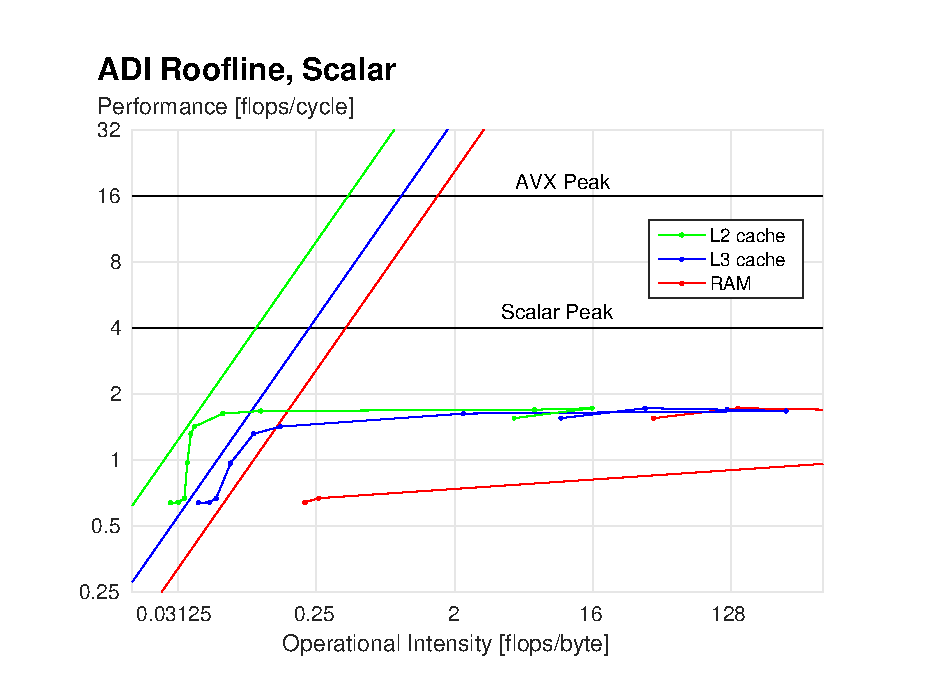
\includegraphics[width=\linewidth]{./plots/roofline_ADI_scalar.eps}
  \caption{Roofline analysis of the ADI scalar code.}
  \label{fig:roofline_ADI_scalar}
\end{figure}

\begin{figure}[H]\centering
  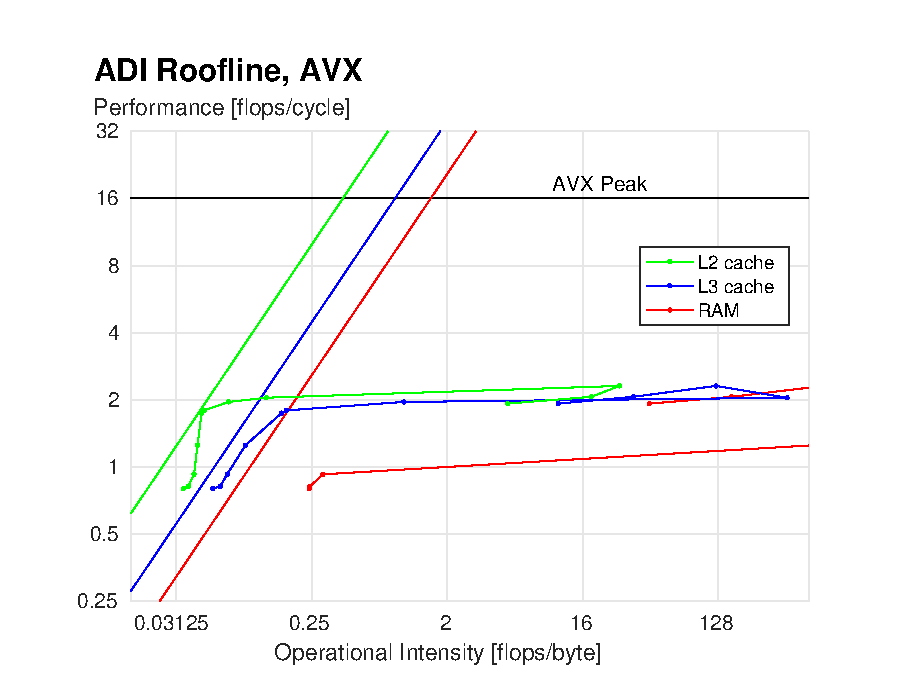
\includegraphics[width=\linewidth]{./plots/roofline_ADI_AVX.eps}
  \caption{Roofline analysis of the ADI AVX code.}
  \label{fig:roofline_ADI_AVX}
\end{figure}

We can immediately see the shifting of the data points (for which the performance values are the same between data series) to the left as the operational intenisty is calculated for lower levels of cache, because the number of data transfers is greater than for RAM. For both the scalar and AVX revisions, the curves move quite close to the respective cache bandwidth rooflines for medium to large problem sizes, at one point becoming almost perfectly tangential to the L2 memory bound. This is a good indication that the low percentage of peak performance achieved is due to the problem being memory bound deeper in the cache structure than was captured with a stadard RAM only analysis, and demonstrates that the code is already close to optimal for the current level of memory transfer.

\mypar{Runtime}
The runtimes for the three revisions of the ADI code are shown in Fig. \ref{fig:runtime_ADI}. Both the scalar and AVX revisions give an additional speedup, but the difference is very small between the two optimized revisions, giving strong evidence for the compiler having performed vectorizations even before the manual AVX instrinsics were introduced. Average runtime speedups of 6.4X and 7.1X with maximums of 8.2X and  9.4X were measured for the scalar and AVX codes, respectively, against the baseline.

\begin{figure}\centering
  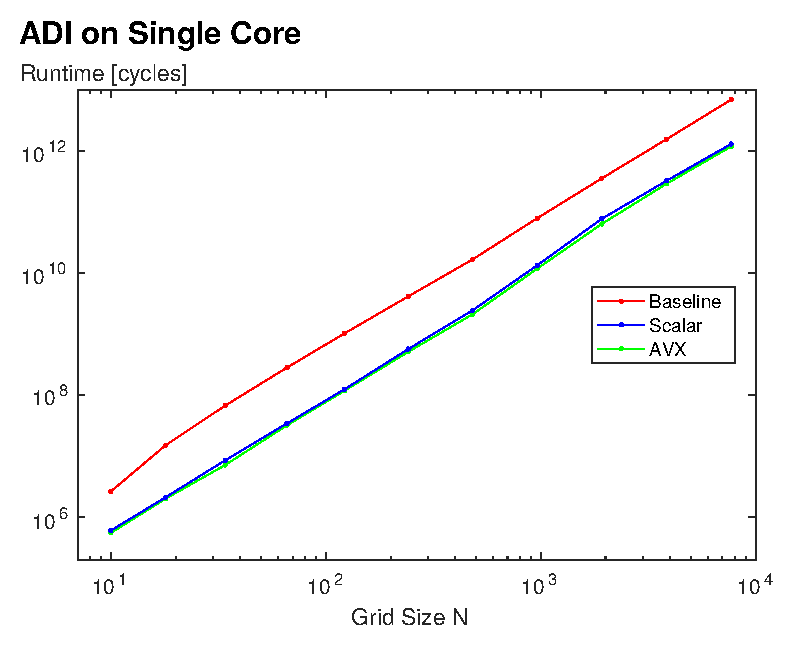
\includegraphics[width=\linewidth]{./plots/runtime_ADI.eps}
  \caption{Runtime analysis of the ADI code.}
  \label{fig:runtime_ADI}
\end{figure}

\mypar{Scaling}
Strong scaling speedup of the ADI code is shown in Fig. \ref{fig:scaling_strong_ADI}. As mentioned, the benchmarking was performed on a single node of Piz Daint, with a total of 12 physical cores present. However, the number of OpenMP threads spawned was vaired between 1 and 24 to also test the possibility of gains from Intel's Hyper-threading technology. Reasonable scaling performance can be seen up to the physically present 12 cores, with almost no further change in runtime for of the Hyper-threaded runs, as would be expected for a problem that is constrained by memory bendwidths in the cache.

\begin{figure}\centering
  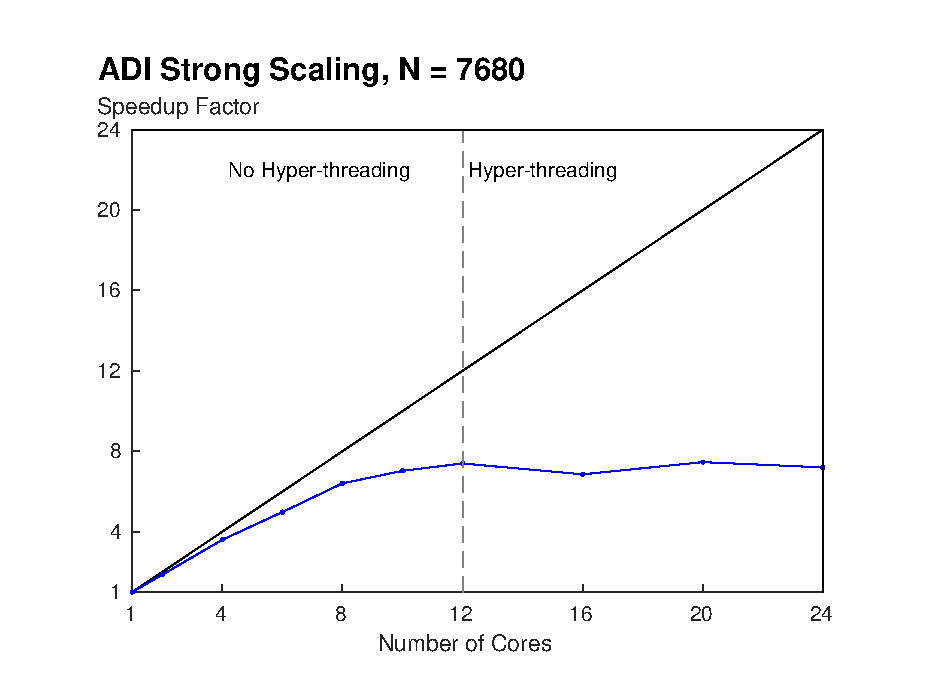
\includegraphics[width=\linewidth]{./plots/scaling_strong_ADI.eps}
  \caption{Strong Scaling analysis of the ADI OpenMP code.}
  \label{fig:scaling_strong_ADI}
\end{figure}

In Fig. \ref{fig:scaling_weak_ADI} can be seen the results of the complementary weak scaling experiment, which was conducted only on 1 to 12 cores. In both cases we see acceptable scaling performance, but with a notable loss in efficiency for higher numbers of cores. This is potentially due to the Non-Uniform Memory Access (NUMA) nature of the Piz Daint nodes, which would necessitate potentially longer memory access times for thread numbers greater than the six cores present in a single socket. It is also noted that the dimensional splitting nature of the ADI algorithm requires two synchronization barriers in each timestep interation, and these synchronization costs could become more pronounced as the number of threads being synchronized increases.

\begin{figure}[!b]\centering
  \includegraphics[width=\linewidth]{./plots/scaling_weak_ADI.eps}
  \caption{Weak Scaling analysis of the ADI OpenMP code.}
  \label{fig:scaling_weak_ADI}
\end{figure}

\subsection{RW}\label{subsec:RW_results}
Only runtime and scaling analyses of the RW code were conducted and are presented here. Performance and roofline analyses were not carried out because of the ''black box'' nature of the PRNGs in the code, which render it essentially impossible to measure, or even usefully approximate, the number and type of operations which occur during the simulation.

\mypar{Runtime}
In Fig. \ref{fig:runtime_RW} is shown the runtime data for the RW codes, with successive speedup being again observed for both the scalar and AVX revisions. Average runtime speedups of 16.5X and 34.2X with maximums of 29.8X and 58.4X were measured for the scalar and AVX codes, respectively, against the baseline. Interestingly, a significant kink is seen in the scalar runtime as the problem size become larger than can be held in L3 cache, but such a strong feature is not seen in either the baseline or AVX codes. This would seem to indicate that the use of manual AVX instrinisics somehow allowed the compiler to better pipeline the memory accesses compared to the scalar code. It is also noted that the largest runtime improvements are found for the smallest inputs, with decreasing returns for large problems as the memory transfer time cuts into the benefits of the optimizations.

\begin{figure}\centering
  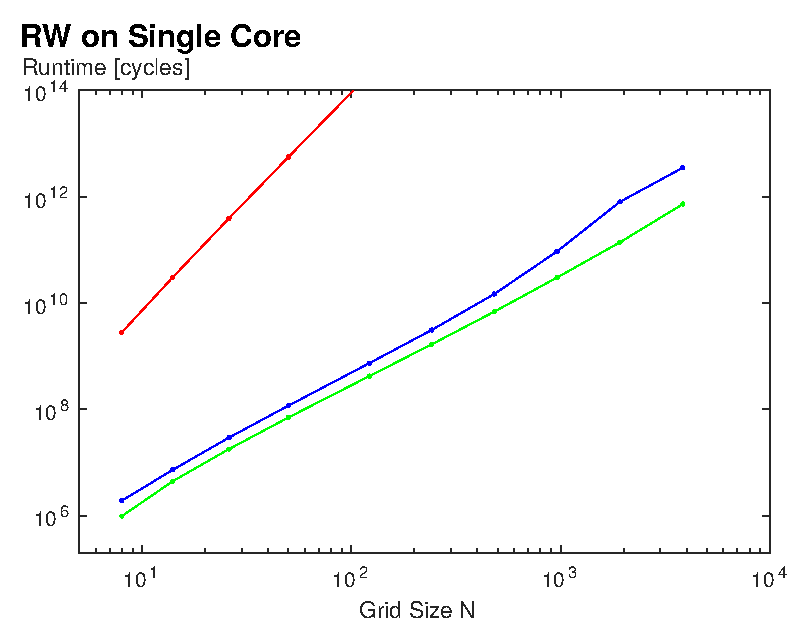
\includegraphics[width=\linewidth]{./plots/runtime_RW.eps}
  \caption{Runtime analysis of the RW code.}
  \label{fig:runtime_RW}
\end{figure}

\mypar{Scaling}
The strong scaling data for the RW code is presented in Fig. \ref{fig:scaling_strong_RW}, again varying over 1 to 24 threads on a single Piz Daint node. We see excellent and consistent scaling scharacteristics up to the 12 physical cores present on the processor, and even achieve a small amount of additional speedup in the Hyper-threading region. This would indicate that the algorithm is not entirely memory \textbf{or} compute bound, but rather limited by dependencies between operations. This means that spawning more threads allows additional independent memory movement and instruction level parallelism to be realized, giving a small amount of further speedup.

\begin{figure}\centering
  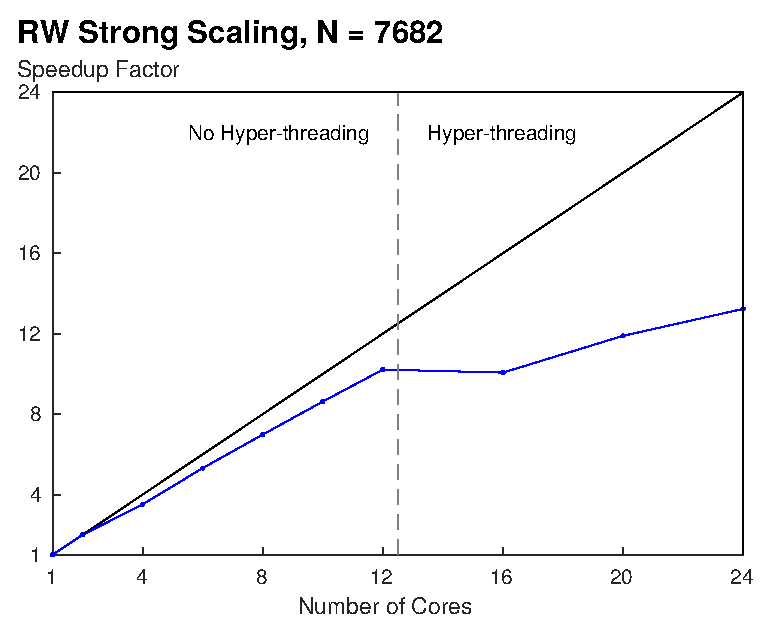
\includegraphics[width=\linewidth]{./plots/scaling_strong_RW.eps}
  \caption{Strong Scaling analysis of the RW OpenMP code.}
  \label{fig:scaling_strong_RW}
\end{figure}

From the weak scaling data shown in Fig. \ref{fig:scaling_weak_RW}, the highly consistent scaling efficiency of the code is again observed. This consistent scaling behaviour for all cores of the node would also lend credence to the idea that this algorithm was not memory bound, since as opposed to the drop-off in efficiency seen in the ADI case, the same potential isssues arising from the NUMA node architecture are not observed for the RW code.

\begin{figure}[!b]\centering
  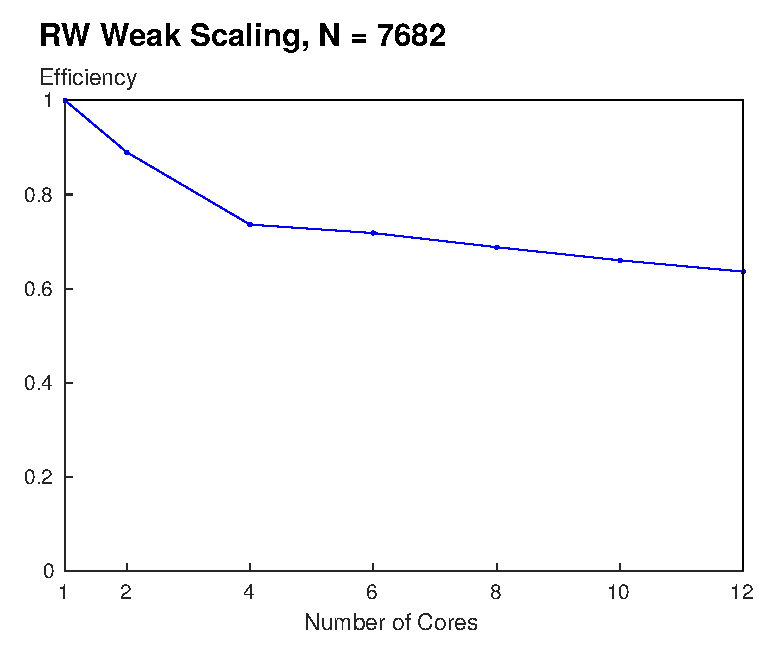
\includegraphics[width=\linewidth]{./plots/scaling_weak_RW.eps}
  \caption{Weak Scaling analysis of the RW OpenMP code.}
  \label{fig:scaling_weak_RW}
\end{figure}


% ----------------------------------------------------------------------
\section{Conclusion}
Numerical simulation of the diffusion equation is an important problem for a broad array of academic fields. As such, optimization and parallelization techniques for efficient implementation of these simulations were presented. The Alternating Direction Implicit and Random Walk algorithms were implemented in C++ with an analytic solution used for verification. Successive scalar optimization, manual AVX vectorization with intrinsics, and OpenMP parallelization were carried out, before the conducting of benchmarking tests on the Piz Daint cluster to determine single-core performance and runtime improvements and as well as single-node strong and weak scaling characteristics.

For the ADI codes, a maximum performance gain of 4.8X and maximal runtime speedup of approximately 9.4X were achieved. Scalar optimizations such as precompuations and loop-unrolling to promote data reuse were found to have siginificant effects on the runtime, while manual vectorization wtih AVX intrinsics provided only minimal additional benefit, most likely due to the automatic vectorizing capabilities of the compiler. A strong scaling efficiency of 61.6\% was measured for 12 threads, corresponding to the 12 phsycial cores of the processor, with no additional benefit gained from Hyper-threading.

For the RW codes, an average runtime improvement of 34.2X, reaching a maximum of 58.4X for small inputs, was observed. The largest bottleneck for this algorithm was found to be the generation of random numbers, and so the choice of PRNG and optimizations which reduced the number of calls to the selected PRNG were of greatest importance. In particular, using binomially distributed random variables to move particles as groups and using the SSE vectorized PRNG from the Intel MKL VS library to generate four values at a time both greatly reduced the runtime. Manual vectorization with AVX intrinsics was again found to be of marginal effectiveness, in this instance because of the small amount of time that was spent outside of the PRNG calls. Excellent scaling efficiency of 85.1\% on 12 threads was reached, and a small but noteworthy additional speedup was measured when using Hyper-threading.

% ----------------------------------------------------------------------


\begin{thebibliography}{99}

\urlstyle{same}

\bibitem{thomas}{Wikipedia. (2017, May 16). \emph{Tridiagonal matrix algorithm} [Online]. Available: \url{https://en.wikipedia.org/wiki/Tridiagonal_matrix_algorithm}}

\bibitem{daint}{CSCS. (Accessed 2017, Aug). \emph{Piz Daint} [Online]. Available: \url{http://www.cscs.ch/computers/piz_daint/}}

\bibitem{7_cpu}{7-CPU. (Accessed 2017, Aug). \emph{Intel Haswell} [Online]. Available: \url{http://www.7-cpu.com/cpu/Haswell.html}}

\bibitem{manual_intel}{Intel Corporation. (2016, Jun). \emph{Intel 64 and IA-32 Architectures Optimization Reference Manual} [Online]. Available: \url{https://www.intel.com/content/www/us/en/architecture-and-technology/64-ia-32-architectures-optimization-manual.html}}

\bibitem{sitmo}{T. van den Berg. (Accessed 2017, Aug). \emph{High Quality C++ Parallel Random Number Generator} [Online]. Available: \url{https://www.sitmo.com/?p=1206}}

\bibitem{transpose}{user2927848. (2016, Mar 23). \emph{m256d TRANSPOSE4 Equivalent} [Online]. Available: \url{https://stackoverflow.com/questions/36167517/m256d-transpose4-equivalent}}

\bibitem{Agner}{A Fog. (2017, May 2). \emph{Instruction tables} [Online]. Available: \url{http://www.agner.org/optimize/instruction_tables.pdf}}

\bibitem{affinity}{Intel Corporation. (Accessed 2017, Aug). \emph{Thread Affinity Interface (Linux* and Windows*)} [Online]. Available: \url{https://software.intel.com/en-us/node/684320}}

\bibitem{SFMT}{Intel Corporation. (Accessed 2017, Aug). \emph{SFMT19937} [Online]. Available: \url{https://software.intel.com/en-us/node/590406}}

\bibitem{cpu_world}{CPU-World. (Accessed 2017, Aug). \emph{Intel Xeon E5-2690 v3 specifications} [Online]. Available: \url{http://www.cpu-world.com/CPUs/Xeon/Intel-Xeon%20E5-2690%20v3.html}}

\bibitem{ark_intel}{Intel Corporation. (Accessed 2017, Aug). \emph{Intel Xeon Processor E5-2690 v3} [Online]. Available: \url{http://ark.intel.com/products/81713/Intel-Xeon-Processor-E5-2690-v3-30M-Cache-2_60-GHzl}}

\end{thebibliography}

\end{document}
